\newpage
\subsection{Exponentielles Modell}

\subsubsection{Wachstum}
\hfill \break
Jemand hat 25€ am Spaarbuch und bekommt Wöchentich 3\% vom Ersparten dazu.
\hfill \break
$K(t)=\textcolor{red}{25}*\textcolor{blue}{1.03}^t$

\begin{itemize}
    \item \textcolor{red}{25}: Startwert
    \item \textcolor{blue}{1.05}: Wachstrumsfaktor
\end{itemize}

\hfill \break
Darstellung:\\
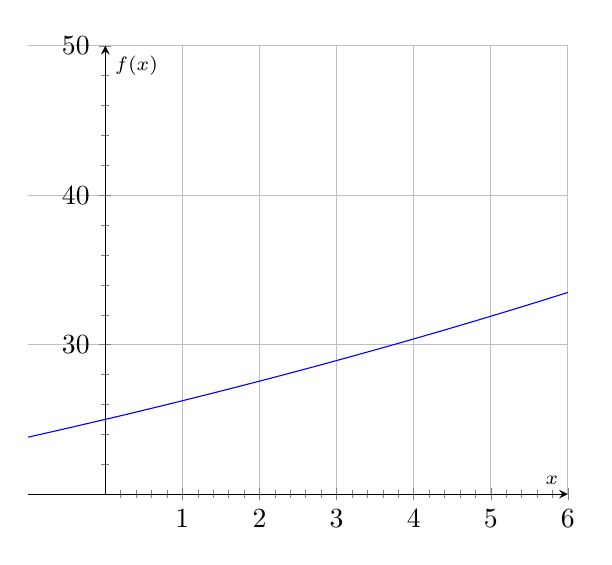
\begin{tikzpicture}[scale=1.0]
    \begin{axis}%
        [
            grid=major,
            xtick={0,1,...,7},
            minor x tick num=4, % 4 minor ticks => 5 subintervals
            xmin=-1,
            xmax=6,
            xlabel={\scriptsize $x$},
            axis x line=middle,
            ytick={10,20,...,50},
            minor y tick num=4,  % 4 minor ticks => 5 subintervals
            ymin=20,
            ymax=50,
            ylabel={\scriptsize $f(x)$},
            axis y line=middle,
            no markers,
            samples=100,
            domain=-6:6,
        ]
        \addplot[blue] (x,{25*1.05^x});
    \end{axis}
\end{tikzpicture}

\newpage
\subsubsection{Zerfall}

\hfill \break
Auf einem Konto Liegen 90€. Es werden monatlich 20\% abgehoben.
\hfill \break
$K(t)=\textcolor{red}{90}*\textcolor{blue}{0.80}^t$

\begin{itemize}
    \item \textcolor{red}{25}: Startwert
    \item \textcolor{blue}{0.80}: Zerfallsfaktor
\end{itemize}

\hfill \break
Darstellung:\\
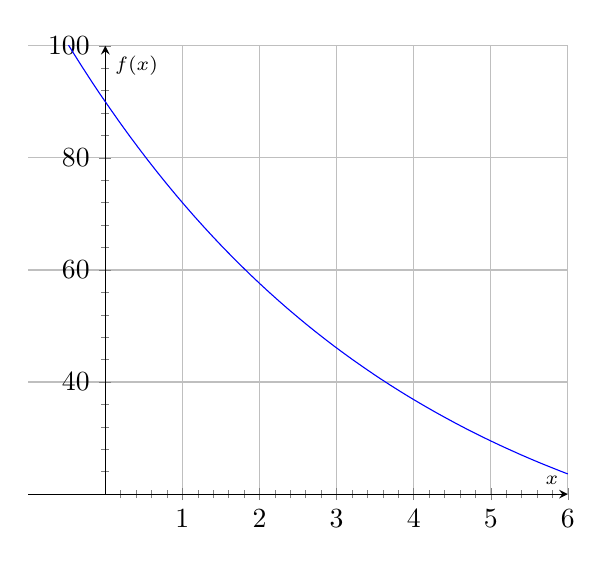
\begin{tikzpicture}[scale=1.0]
    \begin{axis}%
        [
            grid=major,
            xtick={0,1,...,7},
            minor x tick num=4, % 4 minor ticks => 5 subintervals
            xmin=-1,
            xmax=6,
            xlabel={\scriptsize $x$},
            axis x line=middle,
            ytick={20,40,...,100},
            minor y tick num=4,  % 4 minor ticks => 5 subintervals
            ymin=20,
            ymax=100,
            ylabel={\scriptsize $f(x)$},
            axis y line=middle,
            no markers,
            samples=100,
            domain=-6:6,
        ]
        \addplot[blue] (x,{90*0.80^x});
    \end{axis}
\end{tikzpicture}